\documentclass[12pt]{article}

\usepackage{fontspec}
\newfontfamily\handwriting{a-casual-handwritten-pen}[Path=../assets/fonts/,Extension=.ttf,Scale=1.5]
\newfontfamily\comic{Comic Neue}

\usepackage[utf8]{inputenc}
\usepackage{amsmath}
\usepackage{amssymb}
\usepackage{enumitem}
\usepackage{xcolor}
\usepackage{soul}
\usepackage{tikz}
\usepackage[most]{tcolorbox}
\usepackage{titlesec}
\usepackage{multicol}
\usepackage{environ}

\usetikzlibrary{fit, positioning, arrows.meta, decorations.pathreplacing}

% --- Custom Colors ---
\definecolor{primaryblue}{RGB}{42, 111, 151}
\definecolor{exbg}{RGB}{255, 240, 245}
\definecolor{rulebg}{RGB}{232, 245, 233}
\definecolor{highlight}{RGB}{255, 243, 176}
\definecolor{pinkanno}{RGB}{255, 105, 180}
\definecolor{purpleanno}{RGB}{147, 112, 219}
\definecolor{solutionbg}{RGB}{245, 245, 255}

% --- Header Styling ---
\titleformat{\section}{\color{primaryblue}\normalfont\Large\bfseries}{\thesection}{1em}{}
\titleformat{\subsection}{\color{primaryblue}\normalfont\large\bfseries}{\thesubsection}{1em}{}

% --- Friendly Boxes ---
% --- Auto-numbered Example Box ---
\newcounter{examplenum}

\newtcolorbox{friendlyexbox}[1]{
    colback=exbg,
    colframe=pinkanno!50,
    arc=5pt,
    title=\textbf{#1},
    coltitle=black,
    attach title to upper,
    after title={:\quad}
}

\newenvironment{friendlyex}{%
    \refstepcounter{examplenum}%
    \begin{friendlyexbox}{Example \theexamplenum}%
}{%
    \end{friendlyexbox}%
}

\newtcolorbox{friendlyrule}[1]{
    colback=rulebg,
    colframe=primaryblue!30,
    arc=5pt,
    fonttitle=\bfseries,
    title={#1},
    coltitle=primaryblue
}

\newcommand{\funhl}[1]{\sethlcolor{highlight}\hl{#1}}

% --- Show/Hide Solutions ---
\newif\ifshowsolutions

% Uncomment the next line to show solutions.
\showsolutionstrue

\newsavebox{\solutionmeasurebox}

\NewEnviron{solutionbox}{
\ifshowsolutions
\begin{tcolorbox}[
    colback=solutionbg,
    colframe=purpleanno!45,
    arc=5pt,
    title={Solution},
    coltitle=primaryblue,
    fonttitle=\bfseries
]
\BODY
\end{tcolorbox}
\else
\sbox{\solutionmeasurebox}{\begin{minipage}{\dimexpr\linewidth-10pt\relax}\BODY\end{minipage}}
\vspace{\dimexpr\ht\solutionmeasurebox+\dp\solutionmeasurebox+3em\relax}
\fi
}

\begin{document}
\handwriting

\begin{center}
    \Large\textbf{\color{primaryblue}Module 3 Lesson 5\\Inverse Functions} \\
    \vspace{0.2cm}
    \hrule
\end{center}

\section*{Objectives}

\begin{friendlyrule}{In this lesson, we will learn how to}
\begin{itemize}
    \item find the inverse of a relation;
    \item determine whether a function is one-to-one and has an inverse;
    \item verify that two functions are inverses of each other;
    \item find the inverse of a function algebraically;
    \item evaluate and sketch inverse functions from a graph or table.
\end{itemize}
\end{friendlyrule}

\section*{1. Inverse Relations}

\begin{friendlyrule}{Inverse Relation}
Interchanging the first and second coordinate of each ordered pair in a relation produces the \funhl{inverse relation}. If a relation is defined by an equation, interchanging the variables produces an equation of the inverse relation.
\end{friendlyrule}

\begin{friendlyex}{}
Find the inverse relation.
\begin{enumerate}[label=(\alph*)]
    \item Relation: $\{(3,2),(4,1),(5,2)\}$
    \item Relation: $\{(1,2),(3,4),(5,6)\}$
    \item Relation: $y=3x-5$
\end{enumerate}
\end{friendlyex}

\begin{solutionbox}
\textbf{(a)} Swap coordinates: Inverse Relation $=\{(2,3),(1,4),(2,5)\}$.

\textbf{(b)} Swap coordinates: Inverse Relation $=\{(2,1),(4,3),(6,5)\}$.

\textbf{(c)} Swap $x$ and $y$, then solve for $y$:
\[
x=3y-5 \implies x+5=3y \implies y=\frac{x+5}{3}.
\]
\end{solutionbox}

\begin{friendlyrule}{Important Fact}
An inverse relation exists for \textbf{every} function, but the inverse relation is \textbf{not necessarily} a function.
\end{friendlyrule}

\begin{center}
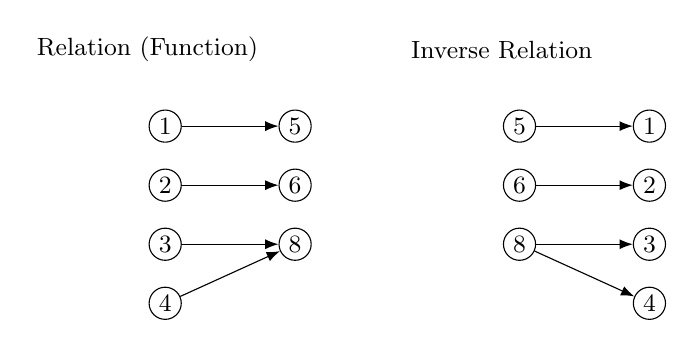
\begin{tikzpicture}[scale=0.75]
\node at (-0.3,4.3) {\small Relation (Function)};
\foreach \i/\y in {1/3,2/2,3/1,4/0} {
    \node[circle,draw,inner sep=1.5pt] (a\i) at (0,\y) {\small \i};
}
\foreach \y/\lab in {3/5,2/6,1/8} {
    \node[circle,draw,inner sep=1.5pt] (b\y) at (2.2,\y) {\small \lab};
}
\draw[-{Latex}] (a1) -- (b3);
\draw[-{Latex}] (a2) -- (b2);
\draw[-{Latex}] (a3) -- (b1);
\draw[-{Latex}] (a4) -- (b1);
\begin{scope}[shift={(6,0)}]
\node at (-0.3,4.3) {\small Inverse Relation};
\foreach \i/\y in {1/3,2/2,3/1} {
    \node[circle,draw,inner sep=1.5pt] (c\i) at (0,\y) {\small \pgfmathparse{int(\i==1?5:(\i==2?6:8))}\pgfmathresult};
}
\foreach \y/\lab in {3/1,2/2,1/3,0/4} {
    \node[circle,draw,inner sep=1.5pt] (d\y) at (2.2,\y) {\small \lab};
}
\draw[-{Latex}] (c1) -- (d3);
\draw[-{Latex}] (c2) -- (d2);
\draw[-{Latex}] (c3) -- (d1);
\draw[-{Latex}] (c3) -- (d0);
\end{scope}
\end{tikzpicture}
\end{center}

Notice: in the Function, both $3$ and $4$ map to $8$. In the Inverse Relation, $8$ maps to \textbf{both} $3$ and $4$ --- so the inverse relation is \textbf{not} a function.

\section*{2. One-to-One Functions}

\begin{friendlyrule}{One-to-One (1--1) Function}
A function is \funhl{one-to-one} if for every $a$ and $b$ in the domain, $a\neq b$ implies $f(a)\neq f(b)$. That is, distinct elements in the domain pair with different elements in the range. Only one-to-one functions have inverses that are also functions.
\end{friendlyrule}

\begin{friendlyrule}{Horizontal Line Test}
If any horizontal line crosses the graph more than once, the function is \textbf{not} one-to-one and does not have an inverse function.
\end{friendlyrule}

\begin{center}
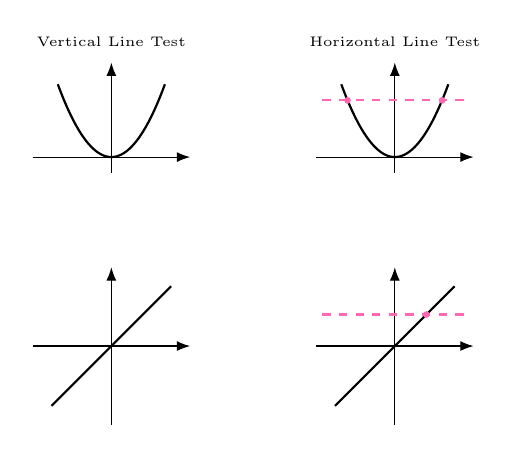
\begin{tikzpicture}[scale=0.4]
\begin{scope}
\node[above] at (0,3.2) {\tiny Vertical Line Test};
\draw[-{Latex}] (-2.5,0) -- (2.5,0);
\draw[-{Latex}] (0,-0.5) -- (0,3);
\draw[thick, domain=-1.7:1.7, samples=40, smooth] plot (\x, {0.8*\x*\x});
\end{scope}
\begin{scope}[shift={(9,0)}]
\node[above] at (0,3.2) {\tiny Horizontal Line Test};
\draw[-{Latex}] (-2.5,0) -- (2.5,0);
\draw[-{Latex}] (0,-0.5) -- (0,3);
\draw[thick, domain=-1.7:1.7, samples=40, smooth] plot (\x, {0.8*\x*\x});
\draw[pinkanno, thick, dashed] (-2.3,1.8) -- (2.3,1.8);
\filldraw[pinkanno] (-1.5,1.8) circle (2.5pt);
\filldraw[pinkanno] (1.5,1.8) circle (2.5pt);
\end{scope}
\begin{scope}[shift={(0,-6)}]
\draw[-{Latex}] (-2.5,0) -- (2.5,0);
\draw[-{Latex}] (0,-2.5) -- (0,2.5);
\draw[thick, domain=-1.9:1.9, samples=30] plot (\x, {\x});
\end{scope}
\begin{scope}[shift={(9,-6)}]
\draw[-{Latex}] (-2.5,0) -- (2.5,0);
\draw[-{Latex}] (0,-2.5) -- (0,2.5);
\draw[thick, domain=-1.9:1.9, samples=30] plot (\x, {\x});
\draw[pinkanno, thick, dashed] (-2.3,1) -- (2.3,1);
\filldraw[pinkanno] (1,1) circle (2.5pt);
\end{scope}
\end{tikzpicture}
\end{center}

The parabola fails the horizontal line test (not one-to-one, no inverse function); the line passes the horizontal line test (one-to-one, has an inverse function).

\begin{friendlyrule}{Domain and Range of an Inverse}
The domain of an inverse, if it exists, is the same as the \funhl{range} of its function. Likewise, the range of the inverse is the same as the \funhl{domain} of the function.
\end{friendlyrule}

\section*{3. Verifying Two Functions are Inverses}

\begin{friendlyrule}{Composition Test}
Two functions $f$ and $g$ are inverses of each other if
\[
(f\circ g)(x)=x \qquad \text{and} \qquad (g\circ f)(x)=x.
\]
We denote the inverse of $f$ by $f^{-1}$.
\end{friendlyrule}

\begin{friendlyex}{}
Determine if $f$ and $g$ are inverses of each other.
\begin{enumerate}[label=(\alph*)]
    \item $f(x)=\dfrac{3}{x+1}\ (x\neq -1)$ and $g(x)=\dfrac3x-1\ (x\neq 0)$
    \item $f(x)=x^3-1$ and $g(x)=\sqrt[3]{x+1}$
\end{enumerate}
\end{friendlyex}

\begin{solutionbox}
\textbf{(a)}
\[
(f\circ g)(x)=f\left(\frac3x-1\right)=\frac{3}{\left(\frac3x-1\right)+1}=\frac{3}{\frac3x}=3\cdot\frac x3=x. \ \checkmark
\]
\[
(g\circ f)(x)=g\left(\frac{3}{x+1}\right)=\frac{3}{\frac{3}{x+1}}-1=(x+1)-1=x. \ \checkmark
\]
Both compositions equal $x$, so $f$ and $g$ \textbf{are} inverses of each other.

\textbf{(b)}
\[
(f\circ g)(x)=\left(\sqrt[3]{x+1}\right)^3-1=(x+1)-1=x. \ \checkmark
\]
\[
(g\circ f)(x)=\sqrt[3]{(x^3-1)+1}=\sqrt[3]{x^3}=x. \ \checkmark
\]
Both compositions equal $x$, so $f$ and $g$ \textbf{are} inverses of each other.
\end{solutionbox}

\section*{4. Finding the Inverse Function Algebraically}

\begin{friendlyrule}{Steps to Find an Inverse Function}
\begin{enumerate}
    \item Rewrite the function in terms of $y$.
    \item Interchange $x$ and $y$.
    \item Solve for $y$.
    \item Rewrite using inverse notation $f^{-1}(x)$.
\end{enumerate}
\end{friendlyrule}

\begin{friendlyex}{}
Find the inverse of $f(x)=4x-5$.
\end{friendlyex}

\begin{solutionbox}
\[
y=4x-5 \implies x=4y-5 \implies x+5=4y \implies y=\frac{x+5}{4}.
\]
\[
\boxed{f^{-1}(x)=\frac{x+5}{4}}
\]
\end{solutionbox}

\begin{friendlyex}{}
Find the inverse function, if it exists.
\begin{enumerate}[label=(\alph*)]
    \item $f(x)=\dfrac{5x+3}{2}$
    \item $g(x)=\dfrac{3x+4}{x-5}\ (x\neq 5)$
    \item $h(x)=5x^2+4\ (x\geq 0)$
\end{enumerate}
\end{friendlyex}

\begin{solutionbox}
\textbf{(a)}
\[
x=\frac{5y+3}{2} \implies 2x=5y+3 \implies 2x-3=5y \implies y=\frac{2x-3}{5}.
\]
\[
\boxed{f^{-1}(x)=\frac{2x-3}{5}}
\]

\textbf{(b)}
\[
x=\frac{3y+4}{y-5} \implies x(y-5)=3y+4 \implies xy-5x=3y+4.
\]
\[
xy-3y=5x+4.
\]
\[
y(x-3)=5x+4 \implies y=\frac{5x+4}{x-3}.
\]
\[
\boxed{g^{-1}(x)=\frac{5x+4}{x-3}\ (x\neq 3)}
\]

\textbf{(c)} Since $x\geq 0$, the range of $h$ is $y\geq 4$, so the domain of $h^{-1}$ is $x\geq 4$.
\[
x=5y^2+4 \implies x-4=5y^2 \implies y^2=\frac{x-4}{5} \implies y=\sqrt{\frac{x-4}{5}}
\]
(taking the positive root, since $y=x\geq 0$ originally).
\[
\boxed{h^{-1}(x)=\sqrt{\frac{x-4}{5}}\ (x\geq 4)}
\]
\end{solutionbox}

\section*{5. Evaluating an Inverse from a Graph or Table}

\begin{friendlyrule}{Reading $f^{-1}(a)$ from a Graph}
$f^{-1}(a)=b$ means $f(b)=a$. On the graph of $f$, locate $a$ on the $y$-axis and read off the corresponding $x$-value.
\end{friendlyrule}

\begin{friendlyex}{}
Use the graph of $f(x)$ below to estimate the following.
\begin{enumerate}[label=(\alph*)]
    \item $f^{-1}(3)$
    \item $f^{-1}(2)$
\end{enumerate}

\begin{center}
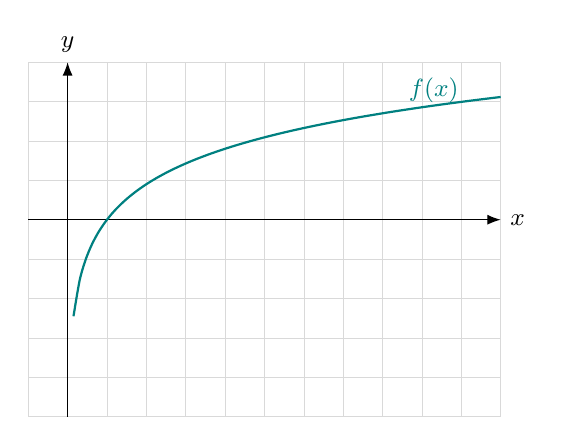
\begin{tikzpicture}[scale=0.5]
\draw[step=1, gray!30, very thin] (-1,-5) grid (11,4);
\draw[-{Latex}] (-1,0) -- (11,0) node[right] {\small $x$};
\draw[-{Latex}] (0,-5) -- (0,4) node[above] {\small $y$};
\draw[teal, thick, domain=0.15:11, samples=70, smooth] plot (\x, {1.3*ln(\x)});
\node[teal] at (9.3,3.3) {\small $f(x)$};
\end{tikzpicture}
\end{center}
\end{friendlyex}

\begin{solutionbox}
\textbf{(a)} Find where the graph has height $y=3$: this occurs at approximately $x=9$. So $f^{-1}(3)\approx 9$.

\textbf{(b)} Find where the graph has height $y=2$: this occurs at approximately $x=4$. So $f^{-1}(2)\approx 4$.
\end{solutionbox}

\begin{friendlyex}{}
Use the table below to evaluate the following.

\begin{center}
\begin{tabular}{|c|c|c|c|c|c|c|}
\hline
$t$ & $0$ & $4$ & $5$ & $10$ & $12$ & $16$ \\
\hline
$H(t)$ & $10$ & $22$ & $30$ & $48$ & $25$ & $11$ \\
\hline
\end{tabular}
\end{center}

\begin{enumerate}[label=(\alph*)]
    \item $H^{-1}(48)$
    \item $H^{-1}(11)$
\end{enumerate}
\end{friendlyex}

\begin{solutionbox}
\textbf{(a)} Find $t$ such that $H(t)=48$: from the table, $H(10)=48$. So $H^{-1}(48)=10$.

\textbf{(b)} Find $t$ such that $H(t)=11$: from the table, $H(16)=11$. So $H^{-1}(11)=16$.
\end{solutionbox}

\section*{6. Sketching an Inverse from a Graph}

\begin{friendlyrule}{Reflection Property}
The graphs of a function and its inverse are reflections of one another across the line $y=x$.
\end{friendlyrule}

\begin{center}
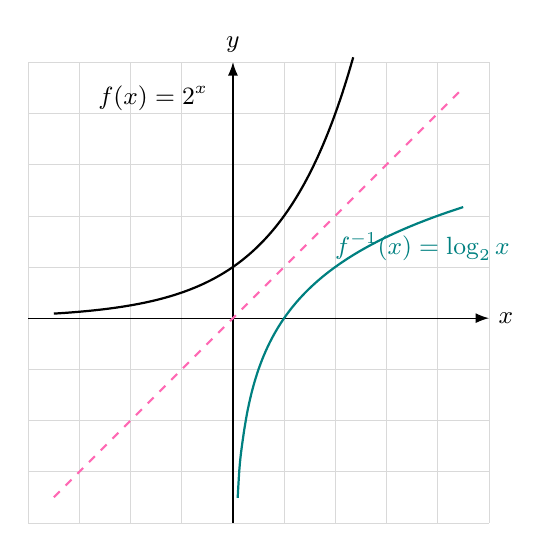
\begin{tikzpicture}[scale=0.65]
\draw[step=1, gray!30, very thin] (-4,-4) grid (5,5);
\draw[-{Latex}] (-4,0) -- (5,0) node[right] {\small $x$};
\draw[-{Latex}] (0,-4) -- (0,5) node[above] {\small $y$};
\draw[pinkanno, dashed, thick] (-3.5,-3.5) -- (4.5,4.5);
\draw[thick, domain=-3.5:2.35, samples=60, smooth] plot (\x, {2^\x});
\node[anchor=east] at (-0.3,4.3) {\small $f(x)=2^x$};
\begin{scope}
\clip (0.05,-3.5) rectangle (4.5,4.5);
\draw[teal, thick, domain=0.05:4.5, samples=60, smooth] plot (\x, {ln(\x)/ln(2)});
\end{scope}
\node[teal] at (3.7,1.4) {\small $f^{-1}(x)=\log_2 x$};
\end{tikzpicture}
\end{center}

Notice that $f$ passes through $(0,1)$, while its reflection $f^{-1}$ passes through $(1,0)$ --- every point $(a,b)$ on $f$ corresponds to a point $(b,a)$ on $f^{-1}$.

\section*{Summary}

\begin{friendlyrule}{Key Ideas}
\begin{itemize}
    \item The inverse relation swaps the coordinates of every ordered pair (or interchanges $x$ and $y$ in an equation); every function has an inverse relation, but that relation is not always a function.
    \item A function is \textbf{one-to-one} if it passes the horizontal line test; only one-to-one functions have an inverse that is also a function.
    \item The domain of $f^{-1}$ equals the range of $f$, and the range of $f^{-1}$ equals the domain of $f$.
    \item $f$ and $g$ are inverses exactly when $(f\circ g)(x)=x$ and $(g\circ f)(x)=x$.
    \item To find $f^{-1}$ algebraically: write $y=f(x)$, swap $x$ and $y$, then solve for $y$.
    \item The graphs of $f$ and $f^{-1}$ are reflections of each other across the line $y=x$.
\end{itemize}
\end{friendlyrule}

\end{document}
